\chapter{Maschinelles Lernen}
Das maschinelle Lernen ist ein Teilgebiet der künstlichen Intelligenz und übernimmt Aufgaben die typischerweise menschliche Intelligenz erfordern. Sie soll dabei helfen Muster und Gesetzmäßigkeiten in Datensätzen zu erkennen. Aus vorhandenen Daten wird durch Algorithmen künstliches Wissen generiert.

\section{Methoden maschinellen Lernens}
Maschinelles Lernen lässt sich nach [\href{https://www.talend.com/de/resources/maschinelles-lernen}{talend.com}] in vier Methoden unterteilen. Die in den folgenden Kapiteln näher betrachtet werden.

\subsection{Überwachtes Lernen}
Bei überwachtem Lernen erhält ein Computer strukturierte Inputs und gewünschte Ergebnisse. Nun muss der Computer Wege finden mit Inputs, um diese Ergebnisse zu erreichen, d.h der Algorithmus versucht eine vorhersage Funktion zu entwickeln. Die Vorhersagen über die unbekannten oder künftigen Daten wird als prädiktive Modellierung bezeichnet.\vspace{0.2cm}

Das überwachte Lernen lässt sich in zwei Arten unterteilen.
\begin{itemize}
	\item Klassifizierung: das Ergebnis ist eine Kategorie, z. B. Gruppenzugehörigkeit
	\item Regression: hier ist das Ergebnis ein realer Wert, z. B. Produktpreis
\end{itemize}

Mittels verschiedener Methoden lassen sich die Ergebnisse vorhersagen. Diese können Entscheidungsbäume, Random-Forest-Algorithmus, lineare Regression, Naive-Bayes-Verfahren, usw. Eignet sich für Probleme der Klassifizierung und Regression.

\subsection{Unüberwachtes Lernen}
Bei diesem Lernen sind keine strukturieren Daten vorhanden, eher legen sie unstrukturiert und unbeschriftet vor. Der Algorithmus muss die Strukturen selbst erkennen. Aus erkannten Mustern und Merkmalen, lassen sich weitere Muster und Korrelationen vorhersagen. Ist, gibt zwei Arten von unüberwachten Lernen.
\begin{itemize}
	\item Clustering: Gruppierung von Daten, weitere lassen sich in bestehende Cluster zuordnen
	\item Assoziation: Regeln in Daten finden, so werden Daten durch Erfahrung definiert
\end{itemize}

Zu diesem Lernen gehören u. a. K-Means, hierarchische Clusteranalyse und Dimensionsreduktion. Mit dieser Methode lassen sich Probleme des Clustering, Dimensionsreduktion und Lernen von Assoziationsregeln.

\subsection{Teilweise überwachtes Lernen}
Es ist ein Hybridverfahren zwischen unüberwachten und überwachten Lernen. Die Rohdaten sind nur teilweise strukturiert und beschriftet. Durch die strukturierten Daten werden die unstrukturierten aufgewertet.\vspace{0.2cm}

Die strukturierten Daten finden anfangs Verwendung, um diese auf Muster und Korrelationen zu untersuchen. Im Anschluss können diese auf die unstrukturierten angewandt werden. Mit dem teilweise überwachten Lernen können Probleme der Klassifizierung und Regression gelöst werden.

\subsection{Bestärktes Lernen}
Ein Computerprogramm interagiert mit einer dynamischen Umgebung. Beim Ausführen bestimmter Aufgaben erhält das Programm gutes oder schlechtes Feedback für die Aktion. Durch die Belohnung und Bestrafung lernt das Programm die richtigen Verhaltensweisen. Belohnungen werden auf zwei verschiedene Arten vergeben.

\begin{itemize}
	\item Monte Carlo: Vergabe erfolgt am Ende
	\item Temporal-Difference-Learning (TD-Learning): Vergabe der Belohnung erfolgt nach jedem Schritt
\end{itemize}

Als Algorithmen sind hier beispielsweise Q-Learning, Deep Q Network (DQN) und State-Action-Reward-State-Action (SARSA) zu nennen.

\section{Algorithmen zum Analysieren von Onlineshop Daten}
Die verwendeten Algorithmen des maschinellen Lernens können durch ihre Ähnlichkeiten gruppiert werden. In den folgenden Kapiteln werden diese wie in [\href{https://machinelearningmastery.com/a-tour-of-machine-learning-algorithms}{machinelearningmastery.com}] diskutiert.

\subsection{Regressionsalgorithmen}
(eng. Regression Algorithms)\vspace{0.2cm}

Durch die interaktive Verwendung eines Fehlmaßes erfolgt eine Verfeinerung des Algorithmus, der Regressionsalgorithmen (eng. Regression Algorithms) befasst sich mit den Beziehungen zwischen Variablen.\vspace{0.2cm}

Wichtige Algorithmen
\begin{itemize}
	\item Ordinary Least Squares Regression (OLSR)
	\item Linear Regression
	\item Logistic Regression
	\item Stepwise Regression
	\item Multivariate Adaptive Regression Splines (MARS)
	\item Locally Estimated Scatterplot Smoothing (LOESS)
\end{itemize}

\subsection{Instanz-basierende Algorithmen}
(Instance-based Algorithms)\vspace{0.2cm}

Algorithmen
\begin{itemize}
	\item k-Nearest Neighbor (kNN)
	\item Learning Vector Quantization (LVQ)
	\item Self-Organizing Map (SOM)
	\item Locally Weighted Learning (LWL)
	\item Support Vector Machines (SVM)
\end{itemize}

\subsection{Regularisierungsalgorithmen}
(eng. Regularization Algorithms)\vspace{0.2cm}

Algorithmen
\begin{itemize}
	\item Ridge Regression
	\item Least Absolute Shrinkage and Selection Operator (LASSO)
	\item Elastic Net
	\item Least-Angle Regression (LARS)
\end{itemize}

\subsection{Entscheidungsbaumalgorithmen}
(eng. Decision Tree Algorithms)\vspace{0.2cm}

Algorithmen
\begin{itemize}
	\item Classification and Regression Tree (CART)
	\item Iterative Dichotomiser 3 (ID3)
	\item C4.5 and C5.0 (different versions of a powerful approach)
	\item Chi-squared Automatic Interaction Detection (CHAID)
	\item Decision Stump
	\item M5
	\item Conditional Decision Trees
\end{itemize}

\subsection{Bayessche Algorithmen}
(eng. Bayesian Algorithms)\vspace{0.2cm}

Algorithmen
\begin{itemize}
	\item Gaussian Naive Bayes
	\item Multinomial Naive Bayes
	\item Averaged One-Dependence Estimators (AODE)
	\item Bayesian Belief Network (BBN)
	\item Bayesian Network (BN)
\end{itemize}

\subsection{Clustering-Algorithmen}
(eng. Clustering Algorithms)\vspace{0.2cm}

Algorithmen
\begin{itemize}
	\item k-Means
	\item k-Medians
	\item Expectation Maximisation (EM)
	\item Hierarchical Clustering
\end{itemize}

\subsection{Lernalgorithmen für Assoziationsregeln}
(eng. Association Rule Learning Algorithms)\vspace{0.2cm}

Algorithmen
\begin{itemize}
	\item Apriori algorithm
	\item Eclat algorithm
\end{itemize}

\subsection{Neuronale Netze}
(eng. Artificial Neural Network Algorithms)\vspace{0.2cm}

Algorithmen
\begin{itemize}
	\item Perceptron
	\item Multilayer Perceptrons (MLP)
	\item Back-Propagation
	\item Stochastic Gradient Descent
	\item Hopfield Network
	\item Radial Basis Function Network (RBFN)
\end{itemize}

\subsection{Depp-Learning-Algorithmen}
(eng Deep Learning Algorithms)\vspace{0.2cm}

Algorithmen
\begin{itemize}
	\item Convolutional Neural Network (CNN)
	\item Recurrent Neural Networks (RNNs)
	\item Long Short-Term Memory Networks (LSTMs)
	\item Stacked Auto-Encoders
	\item Deep Boltzmann Machine (DBM)
	\item Deep Belief Networks (DBN)
\end{itemize}

\subsection{Dimensionsreduktionsalgorithmen}
(eng. Dimensionality Reduction Algorithms)\vspace{0.2cm}

Algorithmen
\begin{itemize}
	\item Principal Component Analysis (PCA)
	\item Principal Component Regression (PCR)
	\item Partial Least Squares Regression (PLSR)
	\item Sammon Mapping
	\item Multidimensional Scaling (MDS)
	\item Projection Pursuit
	\item Linear Discriminant Analysis (LDA)
	\item Mixture Discriminant Analysis (MDA)
	\item Quadratic Discriminant Analysis (QDA)
	\item Flexible Discriminant Analysis (FDA)
\end{itemize}

\subsection{Ensemble-Algorithmen}
(eng. Ensemble Algorithms)\vspace{0.2cm}

Algorithmen
\begin{itemize}
	\item Boosting
	\item Bootstrapped Aggregation (Bagging)
	\item AdaBoost
	\item Weighted Average (Blending)
	\item Stacked Generalization (Stacking)
	\item Gradient Boosting Machines (GBM)
	\item Gradient Boosted Regression Trees (GBRT)
	\item Random Forest
\end{itemize}

\section{Umsetzung der Datenverarbeitung}
%So was wie Daten bereinigen und zusammenführen.
Erste Tests in Sachen Python und Datenanalyse.

\begin{figure}[!ht]
	\centering
	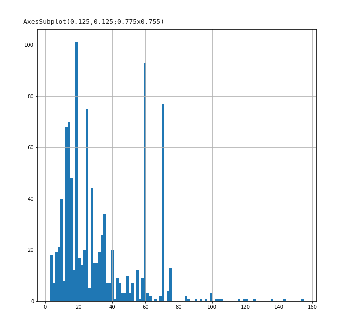
\includegraphics[width=\linewidth]{images/chapter4/first_plot.eps}
	\caption{Anzahl der Bestellung in Abhängigkeit der Warenkorbhöhe}
	\label{img:plot_count_amount}
\end{figure}

\section{Umsetzung der Clusterung}
